\usetikzlibrary{calc}
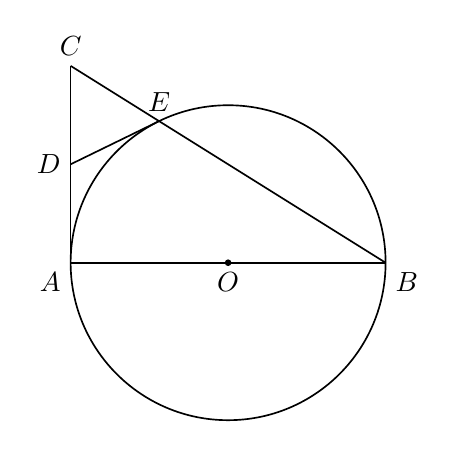
\begin{tikzpicture}[x=1cm,y=1cm,line width=.6pt,font=\normalsize]
\coordinate (O) at (0,0);
\coordinate (A) at (-2,0);
\coordinate (B) at (2,0);
\coordinate (C) at (-2,2.5);
\coordinate (D) at (-2,1.25);
\coordinate (E) at (-0.8764,1.7978);
\draw (O) circle[radius=2cm];
\draw (A)--(B);
\draw (A)--(C);
\draw (B)--(C);
\draw (D)--(E);
\fill (O) circle[radius=1.2pt];
\node[below left] at (A) {$A$};
\node[below right] at (B) {$B$};
\node[below] at (O) {$O$};
\node[above] at (C) {$C$};
\node[left] at (D) {$D$};
\node[above] at (E) {$E$};
\end{tikzpicture}
